\newpage
\printbibliography

\newpage
\addtocontents{toc}{\protect\setcounter{tocdepth}{0}}
\renewcommand{\appendixtocname}{Anhang}
\addappheadtotoc
\renewcommand{\appendixpagename}{Anhang}
\appendices
\appendixpage
\appendixtitleoff
\newcounter{pdfpage}
%%%%%%%%%%%%%%%%%%%%%%%%%%%%%
% Example Appendix with pdf, Page 8
Erster Eintrag: \hyperref[file-1]{Erste Seite}

\includepdf[scale=0.9, frame, pages=3, pagecommand={\thispagestyle{plain}\refstepcounter{pdfpage}\label{file-\thepdfpage}}]{attachments/phwt_style.pdf}

%%%%%%%%%%%%%%%%%%%%%%%%%%%%
\MSonehalfspacing
\newpage
\restoreapp

\newpage
\section*{DIN Normen}

\section*{DIN EN 10002}\label{marker}
Die Versuchsdurchführung erfolgt gemäß DIN EN 10002. Zunächst ist die Probe auszumessen, mit den Vorschriften der Norm zu vergleichen und die Messlänge zu bestimmen.
Danach ist die Probe in die Zugprüfmaschine einzubauen. Die Krafteinleitung erfolgt ausschließlich in axialer Richtung. Zur Messung der Verlängerung wird ein elektronisches
Dehnungsmessgerät, wie in der nachfolgenden Abbildung dargestellt, auf die Probe aufgesetzt mit dem währen der Prüfung kontinuierlich die Probenverlängerung gemessen
wird.


\newpage
\section*{Eigenständigkeitserklärung}
Hiermit versichere ich, dass ich die Hausarbeit selbstständig verfasst und keine anderen als die angegebenen Quellen und Hilfsmittel benutzt habe, alle Ausführungen, die anderen Schriften wörtlich oder sinngemäß entnommen wurden, kenntlich gemacht sind und die Arbeit in gleicher oder ähnlicher Fassung noch nicht Bestandteil einer Studien- oder Prüfungsleistung war.

\vspace{100mm}
% Ort, Datum
\noindent{}STADT, den \today
% Line with 8 cm width
\begin{minipage}[t]{8cm}
\centering \hspace{20mm} \hrulefill \\
% Text under the line
\hspace{20mm}VORNAME NACHNAME
\end{minipage}